% Chapter 4

\chapter{Layout} % Write in your own chapter title
\label{Chapter4} 
\lhead{\emph{Layout}}

In Fig. \ref{fig:layout} si può ammirare il layout finale del Full Adder TSPC.

\begin{figure}[hbt!]
	\centering
	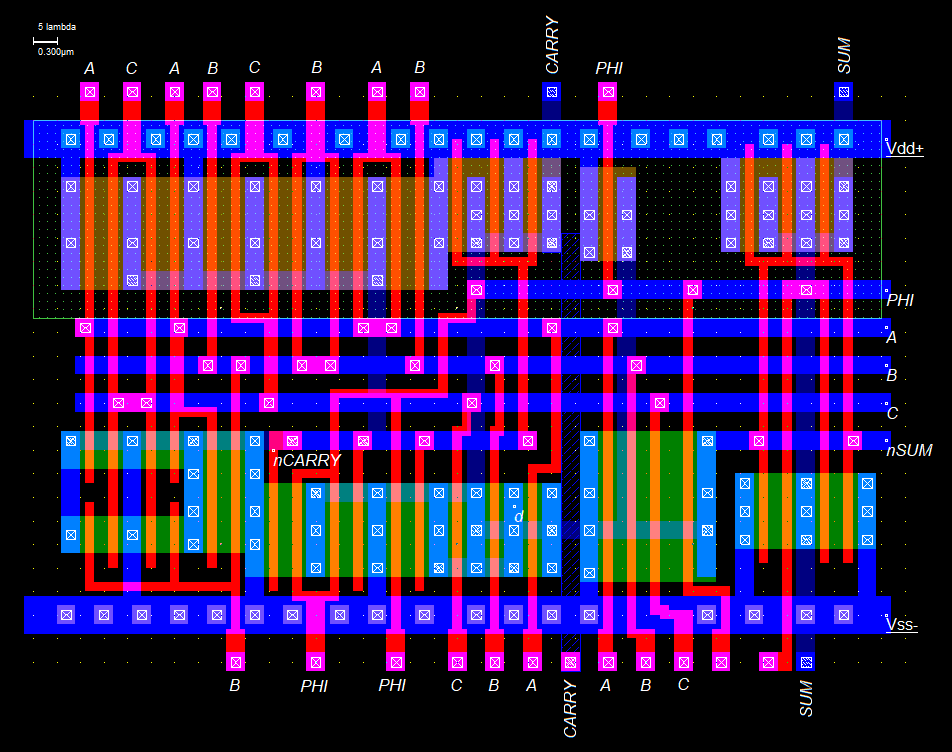
\includegraphics[width=1\textwidth]{figure/Msk_FullDesign.png}
	\caption{Layout finale.}
	\label{fig:layout}
\end{figure}

Vediamo quali sono stati i passi che hanno portato alla sua realizzazione.

\section{Disegno dei singoli stadi}
\label{sec:sec_disegnoStadi}

Un possibile metodo di lavoro prevede di ottenere il circuito finale in maniera progressiva, realizzando un singolo stadio alla volta e unendoli insieme solo una volta che ci si è assicurati della validità di ciascuno di essi, tramite un'opportuna simulazione \textit{post-layout}. Il disegno finale è a sua volta validato da una simulazione dello stesso tipo che, se soddisfacente, sancisce il raggiungimento degli obiettivi prefissati. 

Analizziamo quindi i disegni delle singole parti di circuito riportando alcuni screen tratti da \textit{Microwind} e in cui i colori hanno i seguenti significati:

\begin{itemize}
	\item lo sfondo nero rappresenta il substrato di tipo \textit{p};
	\item le aree verdi sono diffusioni di tipo \textit{n};
	\item le aree verdi a puntini sono diffusioni di tipo \textit{n-well};
	\item le aree rosse costituiscono piste di polisilicio;
	\item le aree blu sono metalizzazioni di tipo \textit{metal 1}; 
	\item i quadrati con la croce all'interno indicano la presenza di un contatto tra livelli differenti.
\end{itemize}

\subsection{Stadio \textit{1}}

In fig. \ref{fig:NMOSnotCarry} si può osservare la realizzazione della parte \textit{n} dello stadio \textit{1} dedicato alla generazione del segnale \textit{!CARRY}, mentre la fig. \ref{fig:PMOSnotCarry} è relativa alla parte \textit{p}. 

Per ciascuno dei due circuiti viene estratta la netlist che, tramite \textit{LTspice}, permette di validare il disegno tenendo conto di tutti i parametri presenti nel modello della tecnologia utilizzata.

\begin{figure}[hbt!]
	\centering
	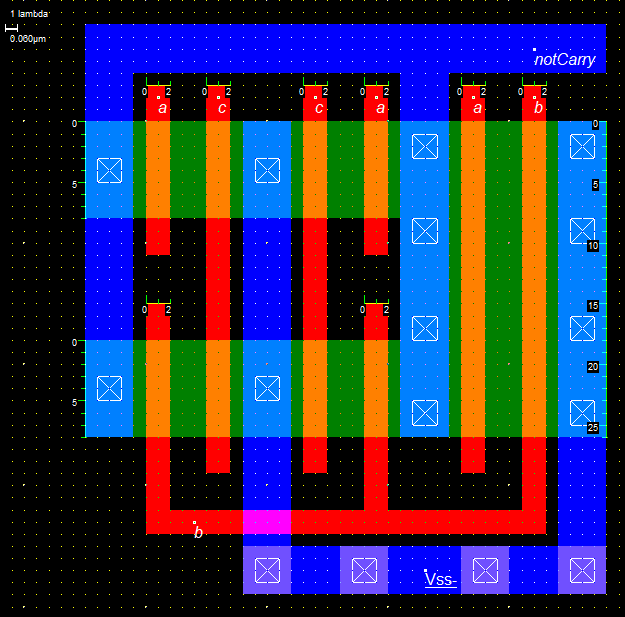
\includegraphics[width=0.5\textwidth]{figure/Msk_NMOS_notCarry_V2.png}
	\caption{Parte \textit{n} dello stadio 1.}
	\label{fig:NMOSnotCarry}
\end{figure} 

\begin{figure}[hbt!]
	\centering
	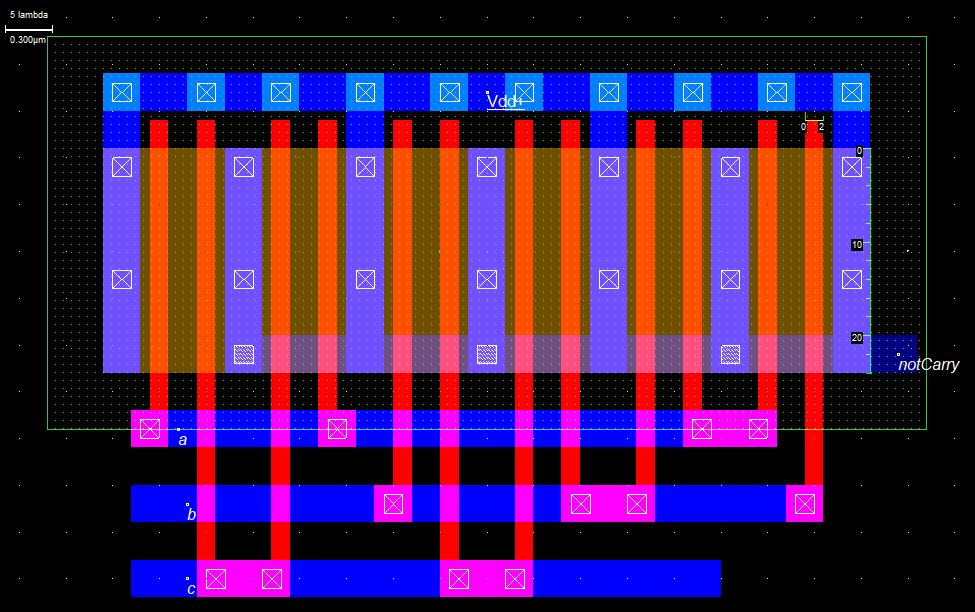
\includegraphics[width=0.7\textwidth]{figure/Msk_PMOS_notCarry_V2.png}
	\caption{Parte \textit{p} dello stadio 1.}
	\label{fig:PMOSnotCarry}
\end{figure} 

Le due parti collegate costituiscono il disegno complessivo dello stadio \textit{1}, raffigurato in fig. \ref{fig:notCarry}, del quale si effettua la validazione procedendo nel modo già descritto. Da tale figura si può notare la scelta di adottare un approccio \textit{standard cell} per la disposizione delle piste di alimentazione e di segnale, come d'altronde viene suggerito nelle specifiche di progetto. In alto e in basso sono quindi presenti due piste orizzontali di \textit{Metal 1} collegate rispettivamente all'alimentazione positiva e negativa. I segnali \textit{A}, \textit{B}, \textit{C} e \textit{notCarry} sono forniti e prelevati in verticale, tramite piste di polisilicio per i primi tre e una pista di \textit{Metal 2} per l'ultimo. Tutti e quattro, assieme a \textit{phi}, sono poi portati nel resto del circuito da alcune piste di \textit{metal 1}, orizzontali, poste tra le parti \textit{n} e le parti \textit{p} di ogni stadio.

\begin{figure}[hbt!]
	\centering
	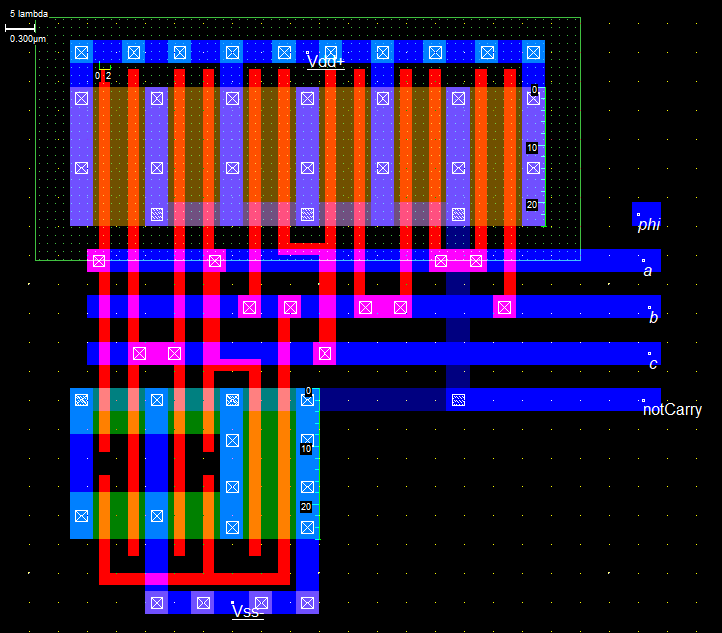
\includegraphics[width=0.5\textwidth]{figure/Msk_NotCarry_V2.png}
	\caption{Disegno dello stadio \textit{1} dedicato alla generazione di \textit{!CARRY}.}
	\label{fig:notCarry}
\end{figure} 

\section{Full design}
\label{sec:sec_fullDesign}






